% 2016 Written PhD Proposal
% Benjamin Rose, advised by Peter Garnavich

%somehow this does not understand \text{}

% \documentclass{aastex}
% \documentclass[preprint2]{aastex}
% default is double spaced `manuscript`, `preprint` or `preprint2` are options
\documentclass[apj, iop]{emulateapj}
\usepackage{graphicx}% Include figure files
\usepackage{color}%for preprints
\usepackage[dvipsnames]{xcolor} %allows for gray links
\usepackage[colorlinks, linkcolor=blue, citecolor=blue, urlcolor=blue]{hyperref}
\usepackage{cleveref} %this allows for \cref{}: http://texblog.org/2013/05/06/cleveref-a-clever-way-to-reference-in-latex/
\usepackage{natbib}
\usepackage{amsmath}  %needed for $\text{}$ and aastex
\usepackage{verbatim}     %for multiline comments with \begin{comment}

\newcommand{\sn}{SNIa}
\newcommand{\todo}[1]{\textbf{\textcolor{red}{#1}}}
\newcommand{\lcdm}{$\Lambda$CDM}     %should use ensure math or something.
\newcommand{\Hubble}{\ensuremath{\text{H}_0}}
\newcommand{\kms}{\ensuremath{~\text{km s}^{-1}}}

% running headers for journal/emulate
\shorttitle{Improved Supernova Distances} 
\shortauthors{Rose}
\slugcomment{\today}

% adds date to aastex versions (emulate has this by default)
% \slugcomment{draft version: \today}
% \slugcomment{}

\begin{document}

% \title{Precision Cosmology: Testing the Cosmological Principle \\with Improved Supernova Distances}
\title{Improved Supernova Distances to Test the Cosmological Principle \\and a Bias in the Hubble Constant}

\author{Benjamin Rose \\{\it advised by} P. M. Garnavich}
\affil{University of Notre Dame, Center for Astrophysics, Notre Dame, IN 46556}
\email{brose3@nd.edu}

% \author{{\it advised by} P. M. Garnavich}

% \and
% \author{{\it advised by} P. M. Garnavich}
% \affil{University of Notre Dame, Center for Astrophysics, Notre Dame, IN 46556}

\begin{abstract} 

Type Ia supernovae (\sn{}) have become a standard cosmological tool, but there
are still improvements needed in this age of precision cosmology.  Cosmology  is
reaching a point where we can now start to test the Cosmological Principle, that
the universe is homogeneous and isotropic on large scales. I have analyzed the
currently available data set of \sn{} to search for bulk flows on a variety of
scales. This analysis confirmed a velocity asymmetry across the sky of $\sim 300~\kms{}$ at
low redshift. We cannot rule out a large-scale bulk flow (dark flow) that could
be caused by quantum entanglement in the early universe. And we show that a
larger \sn{} data set and improved distance precision would provide useful
constraints on any such dark flow. We plan to simulate future large data sets to
determine the optimal observing strategy to constrain the dark flow given the
photometric precision, cadence, and sky coverage possible from LSST and other
future \sn{} surveys.  Furthermore, we will improve the \sn{} distance precision
by correlating Hubble residuals with properties of the local environment around
the supernova. There appears to be some correlation between the global host
properties (e.g. star formation rate, metallicity) and \sn{} luminosity
residuals. There is a controversy as to whether the influence of the local
environment is biasing the best estimates of the Hubble constant (\Hubble{}).
This bias either corrects or continues the tension between \Hubble{} measured
from the CMB or with \sn{}. We will analyze existing high resolution Hubble
Space Telescope images of SDSS host galaxies to see if the stellar properties at
the explosion location correlate with \sn{} luminosity.

\end{abstract}

\maketitle


\section{Introduction}\label{introduction} 

Type Ia supernovae (\sn{}) have been a standard cosmological tool since they
were successfully used to estimate the Hubble constant \citep{Hamuy95,Riess95}
and later to see the accelerated expansion of the Universe
\citep{Riess98,Perlmutter99}. Cosmology is now focusing on precision and with
improved measurements we are able to test its fundamental assumptions. To
perform these tests, both the statistical and systematic uncertainties in \sn{}
distances must be reduced. These measurements will give deeper understanding of
the evolution of the cosmos and the structure and composition of the universe.

The most fundamental assumption is called the Cosmological Principle, that the
universe is homogeneous and isotropic on the largest scales. Simple tests can be
constructed to see if there is a consistent cosmology in all directions. For
these to reach out to distances of gigaparsecs, or of order $0.1$ in redshift,
\sn{} need to have very accurate distance measurements. 
% The needed precision is
% more than a single \sn{} measurement is not going to be able to achieve in the
% foreseeable future. But looking for a change in cosmology means the measurement
% is statistically dominated. 
A single \sn{} at a redshift of 0.1 is not sufficient to reach the accuracy
required to search for a dark flow. But averaging many SNIa measurements in the
same direction on the sky can reduce the statistical uncertainty. Because we are
looking for differences in the cosmology across the sky, systematic errors are
minimized.
More \sn{} are going to come from the massive survey
ongoing and planned for the near future.

As stated above, there is a systematic uncertainty floor in the distance from an
individual \sn{}. \sn{} distances are already corrected for light curve width
and color variations, but new corrections appear to improve distance accuracy,
such as correlations with host galaxy properties or even the local environment
near the explosion. These correlations with the local environment can lead to a
bias in the Hubble constant (\Hubble{}) because of how \sn{} are anchored to
object of known distance. Unlike testing if there is a consistent cosmology in
all directions, looking for a bias in \Hubble{} is dominated by systematic
errors. Finding a bias in \Hubble{} as measured by \sn{} will help with the
tension between this measurement and the value calculated using the CMB.
Performing more analysis of the local environment will advance both supernova
cosmology and cosmology as a whole.


\section{Testing the Cosmological Principle}\label{testing-the-cosmological-principle}

The excepted cosmological model, $\Lambda$CDM, works under a testable assumption
that the universe is isotropic and homogeneous on large scales. These scales are
greater than the size of the present day first acoustic peaks seen in the CMB.
%(\cite{Scrimgeour12} says greater-equal 100h$^{-1}$Mpc in ΛCDM).      
We already know that gravity breaks this isotropic condition on small scales and
produces peculiar motion of galaxies. Specific theories of inflation
\citep[like in][]{MersiniHoughton:2008io} produce a preferred direction in our visible
universe. This direction is due to a slight curvature in space-time from pre-inflation
quantum interactions. Observationally, if this preferred direction exists, we expect to
see a uniform bulk velocity flow that extends outside the local group and into
what $\Lambda$CDM would predict to be a purely isotropic Hubble expansion. Such
a large-scale asymmetry has been called a ``dark flow''
\citep{MersiniHoughton:2008io}. This is a fundamental search to validate our
understanding of the mass-energy make-up of the universe and look for
entanglement from the era before inflation.

\subsection{Previous Tests}\label{previous-tests}

\begin{figure}
	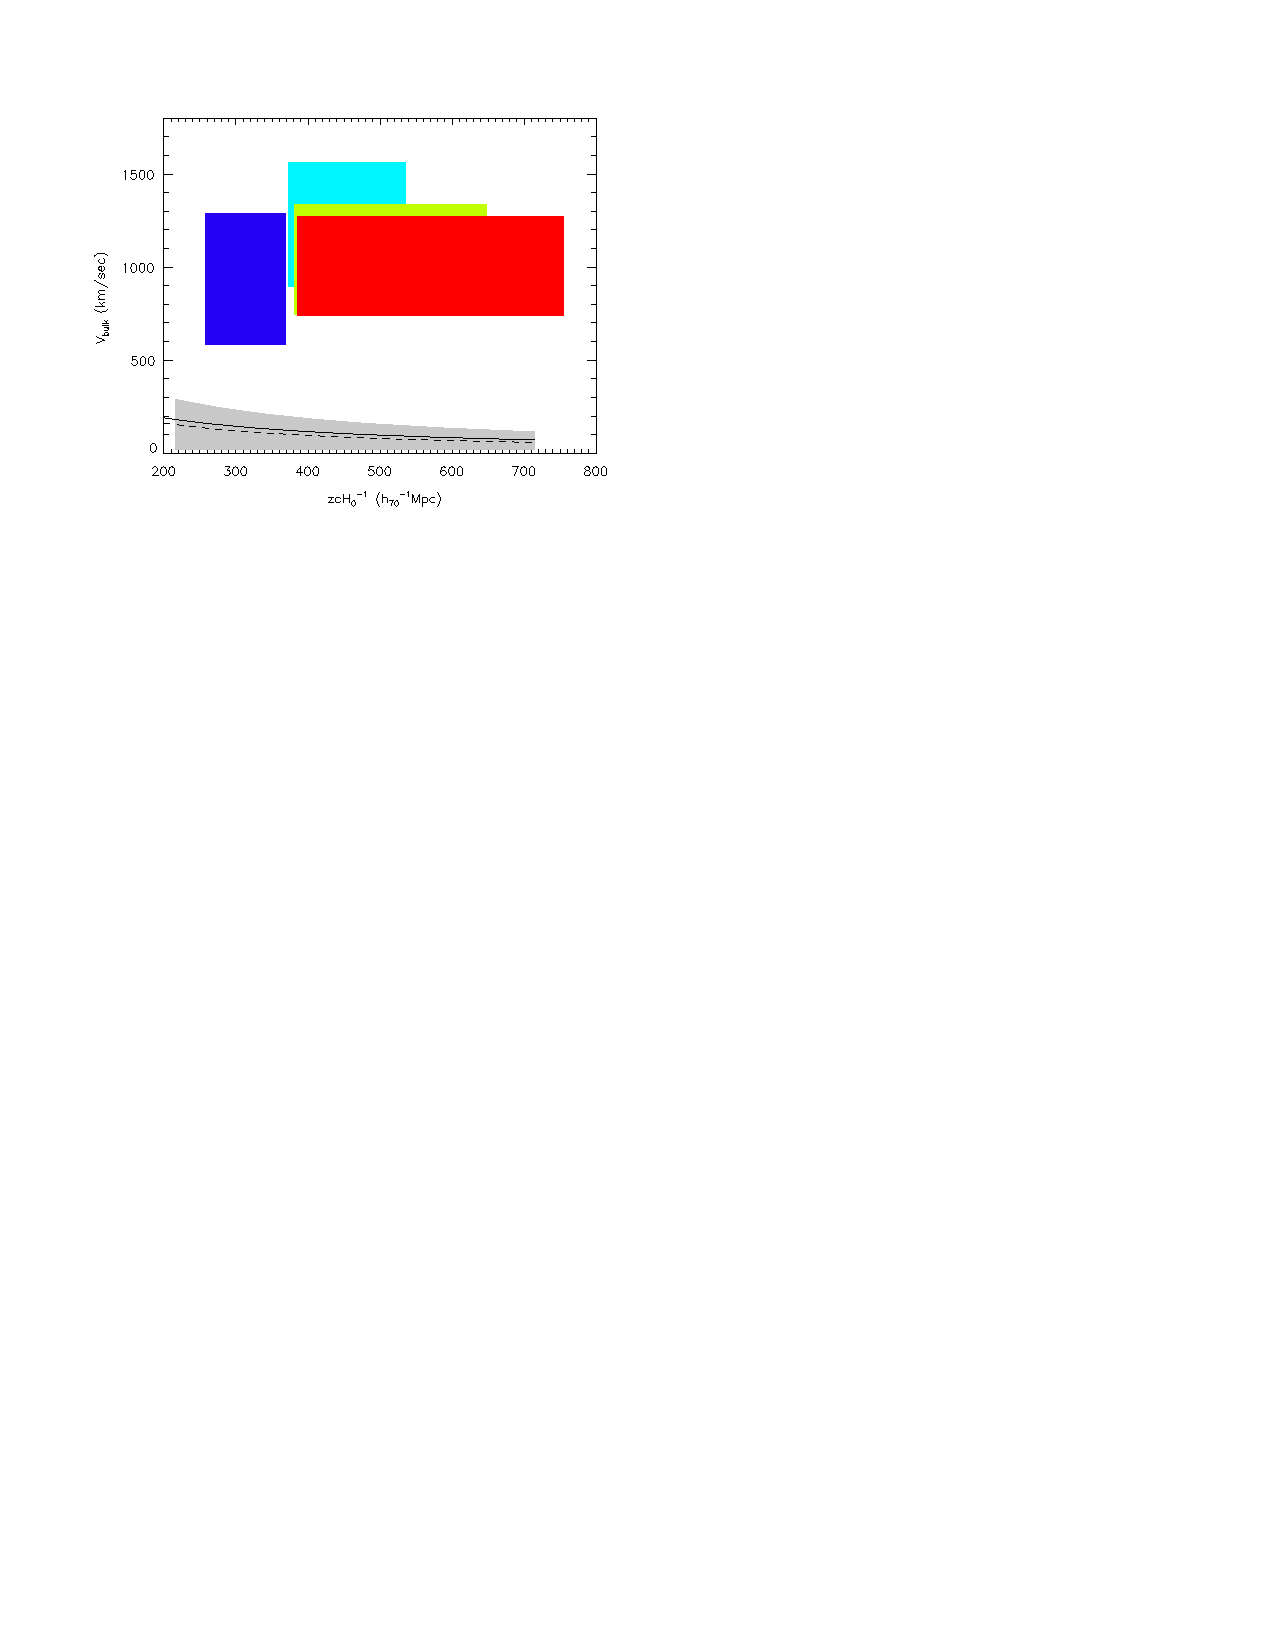
\includegraphics[width=3.2in]{Kashlinsky2010.pdf} 
    \caption{This is the measured bulk flows from the kSZ measurements found in 
    \cite{Kashlinsky10}. The blocks are for $z \leq 0.12$, $0.16$, $0.2$, and 
    $0.25$. A 95\% confidence of a \lcdm{} model is given in the grey-shaded 
    region, with two different priors producing the rms lines.
    Taken from \cite{Kashlinsky10}.}
	\label{f:ksz} 
% Bulk velocity vs. depth from Table 1: blue/cyan/green/red correspond to z \leq
% 0.12/0.16/0.2/0.25; parameters for fits (a) are chosen for brevity.
% Solid/dashed lines correspond to the rms bulk velocity for the concordance
% ΛCDM model for top-hat/Gaussian windows. Black-shaded regions show the
% 95\% confidence level of the model (see KABKE1 for details).
\end{figure}

The universe's isotropic nature has been intensely tested over the last half a
decade with surveys of nearby galaxies \citep{Ma13,Wiltshire:2013dl},
the kinematic Sunyaev- Zel\'{d}ovich (kSZ) effect on distant clusters
\citep{Kashlinsky10,Planckdf}, and with \sn{} data sets \citep[and
others]{Dai11,Feindt13,Rathaus13}. Most searches did not see a bulk flow that
was significantly larger than allowed by \lcdm{} but some saw a bulk flow of
greater than $1000 \kms{}$ out to redshifts of $z = 0.25$, \Cref{f:ksz}. This
measurement cannot be explained by $\Lambda$CDM alone but needs an inflation
theory that predicts this cosmic anisotropy.

\begin{figure}
	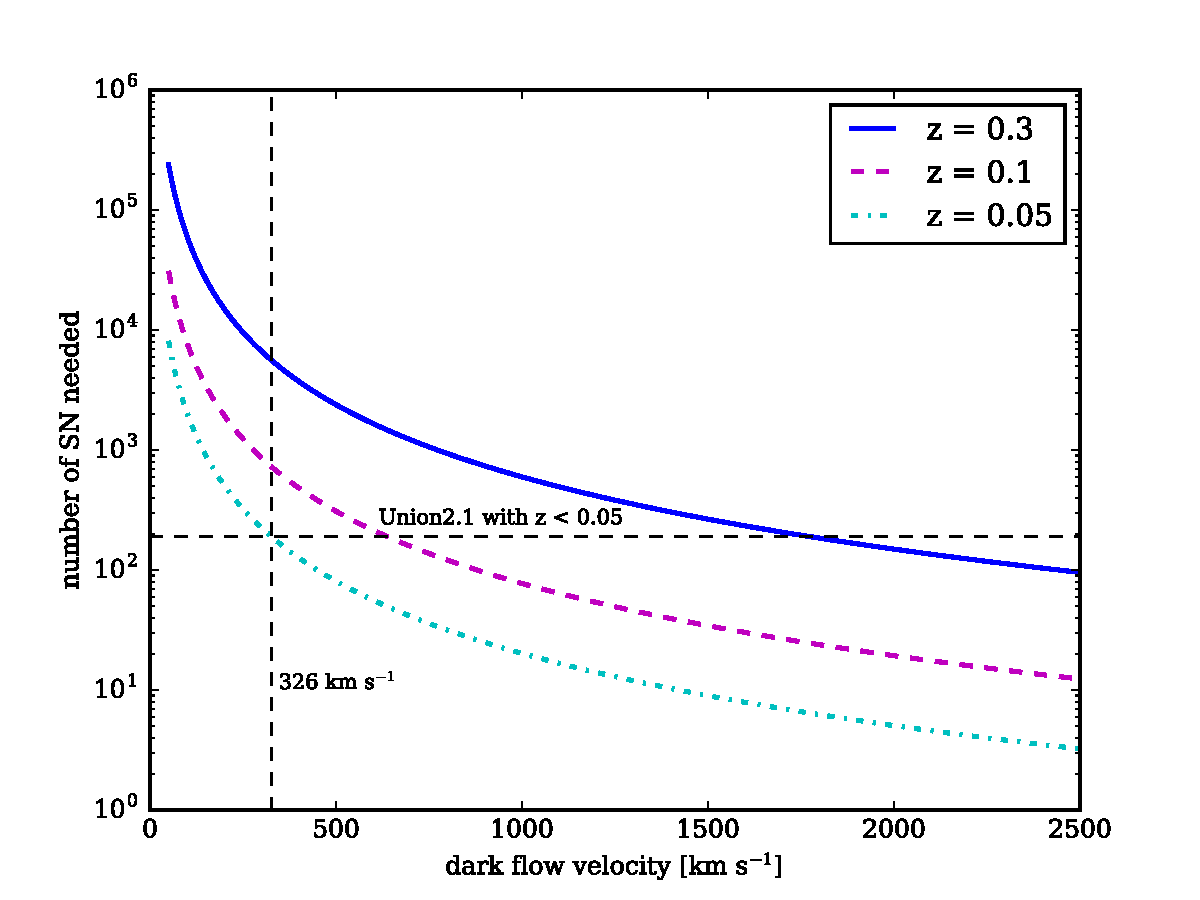
\includegraphics[width=3.2in]{what_dataset_size_v_velocity-2.pdf} 
    \caption{The number of \sn{} needed to see a given dark flow velocity, a
	cosmic scale bulk flow, out to a given redshift. It is seen that Union2.1 
	can detect flows only out to $z=0.05$ and nearly 10$^4$ \sn{} would be 
	needed to see a dark flow out to $z=0.3$. Taken from \cite{Mathews16}}
	\label{f:sn-needed} 
\end{figure}

My work on initial tests of the Cosmological Principle can be found in
\cite{Mathews16}. My contribution was to develop a new method to search for
cosmological asymmetries using the angular separation of a \sn{} and the
direction of the dark flow. We were able to fit the data to a model that
contained both a \lcdm{} cosmology and an bulk flow. If the same bulk flow is
visible across all redshifts, then we have found the dark flow signal. This
analysis was performed on the Union2.1 \sn{} sample \citep{Suzuki12}. We found a
mild bulk flow of $326 \pm 54$ km s$^{-1}$ out to $z = 0.05$. This is consistent
with most past measurements and can be explained by gravitational perturbation
from large scale structure. We also analyzed, for the first time, the large
\sn{} data set from SDSS-II Supernova Survey, both spectroscopic and
photometrically confirmed \sn{} \citep{Campbell13}. This is the largest uniformly
collected \sn{} data set and it had a very even distributed along Stripe
82, $2.5^{\circ}$ wide and about $\sim120^{\circ}$ along the Celestial
Equator. Unfortunately, no measurement was possible because of that limited sky
coverage.

From further analysis we determined that the loss of signal past $z \sim 0.05$
was not from the lack of a dark flow, but from the increase of the uncertainty
in the distance measurements. An order of magnitude reduction of distance
modulus error is needed to see out to $z \sim 0.3$.  This is unattainable with
the current data sets, but it can soon be achieved. First, larger data sets will
reduce the statistical error in \sn{} distances over large parts of the sky.
Looking for a change of cosmology across the sky means any uniform systematics
will be subtracted out and not affect the analysis.  A visual account of the
needed \sn{} to see a given bulk flow can be seen in \Cref{f:sn-needed}. This
large sample size should be achievable with the Large Synoptic Survey Telescope
(LSST) and its uniform photometric reliability of $10 ~\text{mmag}$ across the
visible sky \citep{Ivezic08}. A large, uniform data set will push the
statistical errors at $z\sim 0.3$ to the systematic floor.

\subsection{Future Tests}\label{future-tests}

\begin{comment}
Testing the Cosmological Principle can and should be continued. In search for a
cosmic anisotropy, studies have used galactic surveys, the kinetic Sunyaev-
Zel\'dovich effect, and SNIa, but another possibility is using baryon acoustic
oscillations (BAO). This distance measure is complementary to \sn{} estimates
and subject to smaller systematic uncertainties.
The BAO analysis will follow a similar procedure as developed in
\cite{Mathews16} for SNIa. The test requires a
data set with significant sky coverage, and this is possible with SDSS's eBOSS
and eventually DESI.
\todo{This might want to be removed, do I want to open up questions about BAO?}
\end{comment}

At the end of \cite{Mathews16}, we suggest that LSST might produce a data set
that is able to search for the dark flow. Detailed simulations of LSST-like data
sets are critical in understanding the limits of the survey when applied to the
dark flow problem.  These tests will show if the combination of LSST's
measurement precision, cadence, and sky coverage will be able to place limits on
the dark flow.
% sufficient to test for isotropic expansion as
% is the foundation of \lcdm{} and what limits can be placed on the dark flow.
The future space telescope WFIRST may also be able to help in this measurement,
however, its sky coverage will be limited compared with LSST. It has already
been seen that sky coverage produces a bias in the dark flow velocity
\citep{Appleby14} if not obscuring measurements completely \citep{Mathews16}.
Simulations of the combined LSST and WFIRST data sets will produce useful
insights into optimum future surveys.

Since the analysis method is written, getting a good simulated LSST \sn{} data
set is the hardest part. Telescope uncertainties and project goals have been
stated, but these need to be transitioned, with any errors propagated, into
positions, redshifts, and distances. The hardest part will be redshift. The
community will not be able to get spectra of the hosts at the rate that LSST
will find \sn, reducing the rate of cosmologically usable \sn. One possible way
to get more usable \sn is through the ever improving photometric redshifts
measurements \citep{Kind13}. We don't know what clever new techniques will allow
for more usable data in the future. Anther difficulty is that follow up
telescopes in different locations than LSST, the footprint of the cosmologically
useful \sn{} might be different than LSST's footprint. These and others survey
complexities will need to be taken into account for any accurate modeling of
what can be done with LSST \sn{}.

\begin{comment}
This project is going to push the edge of detection. To get this correct, the
noise will need to be fully understood. A systematic approach is need, going
from  strong signals with unrealistically perfect data to realistic noisy and
incomplete data.  
\end{comment}

Large surveys are being leveraged to reduce the statistical uncertainties in the
distance measurement of \sn{}. With this decreased uncertainty, we will be able
to test the Cosmological Principle and check to see if cosmology is truly
constant no matter where you look.

% \section{Standardizing type Ia
% supernova}\label{standardizing-type-ia-supernova}
\section{Testing for a Bias in the Hubble constant} % (fold)
\label{sec:Hubble_Bias}

The Hubble constant is simply the slope of the relationship between velocity and
distance. Like many aspects of astronomy, measuring distance is the hardest part
of this process. \Hubble{} cannot be measured locally because gravitation from
neighboring galaxies and clusters create relatively large bulk motions. To
measure distances of the whole of the cosmos one needs to rely on the
``distance ladder.''  This is where astronomers start with known distances and
climb their way out to greater and greater distances by using different
measurement techniques along the way. If an anchoring of two techniques is not
consistent with the individual techniques themselves, then a bias can arise.
This is likely to appear if two measurements only overlap in a particular
subtype of objects.

\subsection{New Standardizations}\label{new-standardizations}

The \sn{} community as a whole is focusing on reducing uncertainty in \sn{}
distances. Knowing distance more precisely will narrow the range for the Hubble
constant, the dark energy equation of state as well as constraining the
Cosmological Principle.

\sn{} are not standard candles, but rather standardizeable candles. Since
\cite{Phillips93} there has been significant work to improve off this basic
correction to the variability in \sn{} absolute luminosity. \sn{} color is also
used to standardize \sn{} and this has allowed them to be used for critical
cosmological measurements \citep{Riess98, Perlmutter99}. Currently well-studied
\sn{} typically have a 15\% error in distance modulus (or 7\% in
distance). So it takes about 50 \sn{} to reduce the statistical error down to a
few percent in brightness, which is near the systematic floor. This floor
is partly caused by limits on photometric calibration and partly by intrinsic
uncertainties in the supernovae themselves.

A significant amount of research, time, and energy is spent on trying to reduce
the scatter in the absolute magnitude of \sn{}. It has been found that a
reduction in this scatter can be achieved if the properties of the \sn{}'s host
galaxy are taken into account. Host mass \citep{Childress13} and host
metallicity \citep{Hayden13} have been seen to reduce this intrinsic scatter.

The idea that these global properties directly affect the \sn{} is too loose, so
the community has started to look at the local environment around
the \sn{}. \cite{Rigault13} looked at \sn{} form the Nearby Supernova Factory
and the host galaxy's $\text{H}_{\alpha}$ within a 1 kpc radius of each \sn{}.
They found a bias in the \sn{} standardized luminosity when they divided their
sample in half based on the measured $\text{H}_{\alpha}$. If there was less
$\text{H}_{\alpha}$ then the average corrected luminosity was also lower.  Also
\cite{Rigault15, Jones15} looked at \sn{} in the Constitution sample with host
galaxy data from {\it GALEX} but they disagree on whether there is or is not a
bias.
%\todo{I can do
%better then  this next sentence. Flesh out the fight a bit, how this effect
%\Hubble{} and what my work will do to help.} 
Sorting this controversy out is critical in improving the estimate of the
Hubble constant.

\subsection{Getting Closer in with HST}\label{hst}

I am currently working with Hubble Space Telescope (HST) images of host galaxies
of \sn{} found during SDSS-II Supernova Survey
\citep{2008AJ....135..338F,2008AJ....135..348S}. HST's small angular resolution
allows for a much smaller definition of local environment. For a galaxy at $z =
0.1$ HST provides a local environment on the scale of $\sim 160~\text{pc}$,
verses the $1~\text{kpc}$ that was used with {\it GALEX} data in
\cite{Jones15,Rigault15}. This can be seen in the comparison between SDSS
(having a simpler angular resolution to {\it GALEX}) and HST images of the host
galaxy of SN 2005fw seen in \Cref{f:galaxy-compare}.

\begin{figure}
	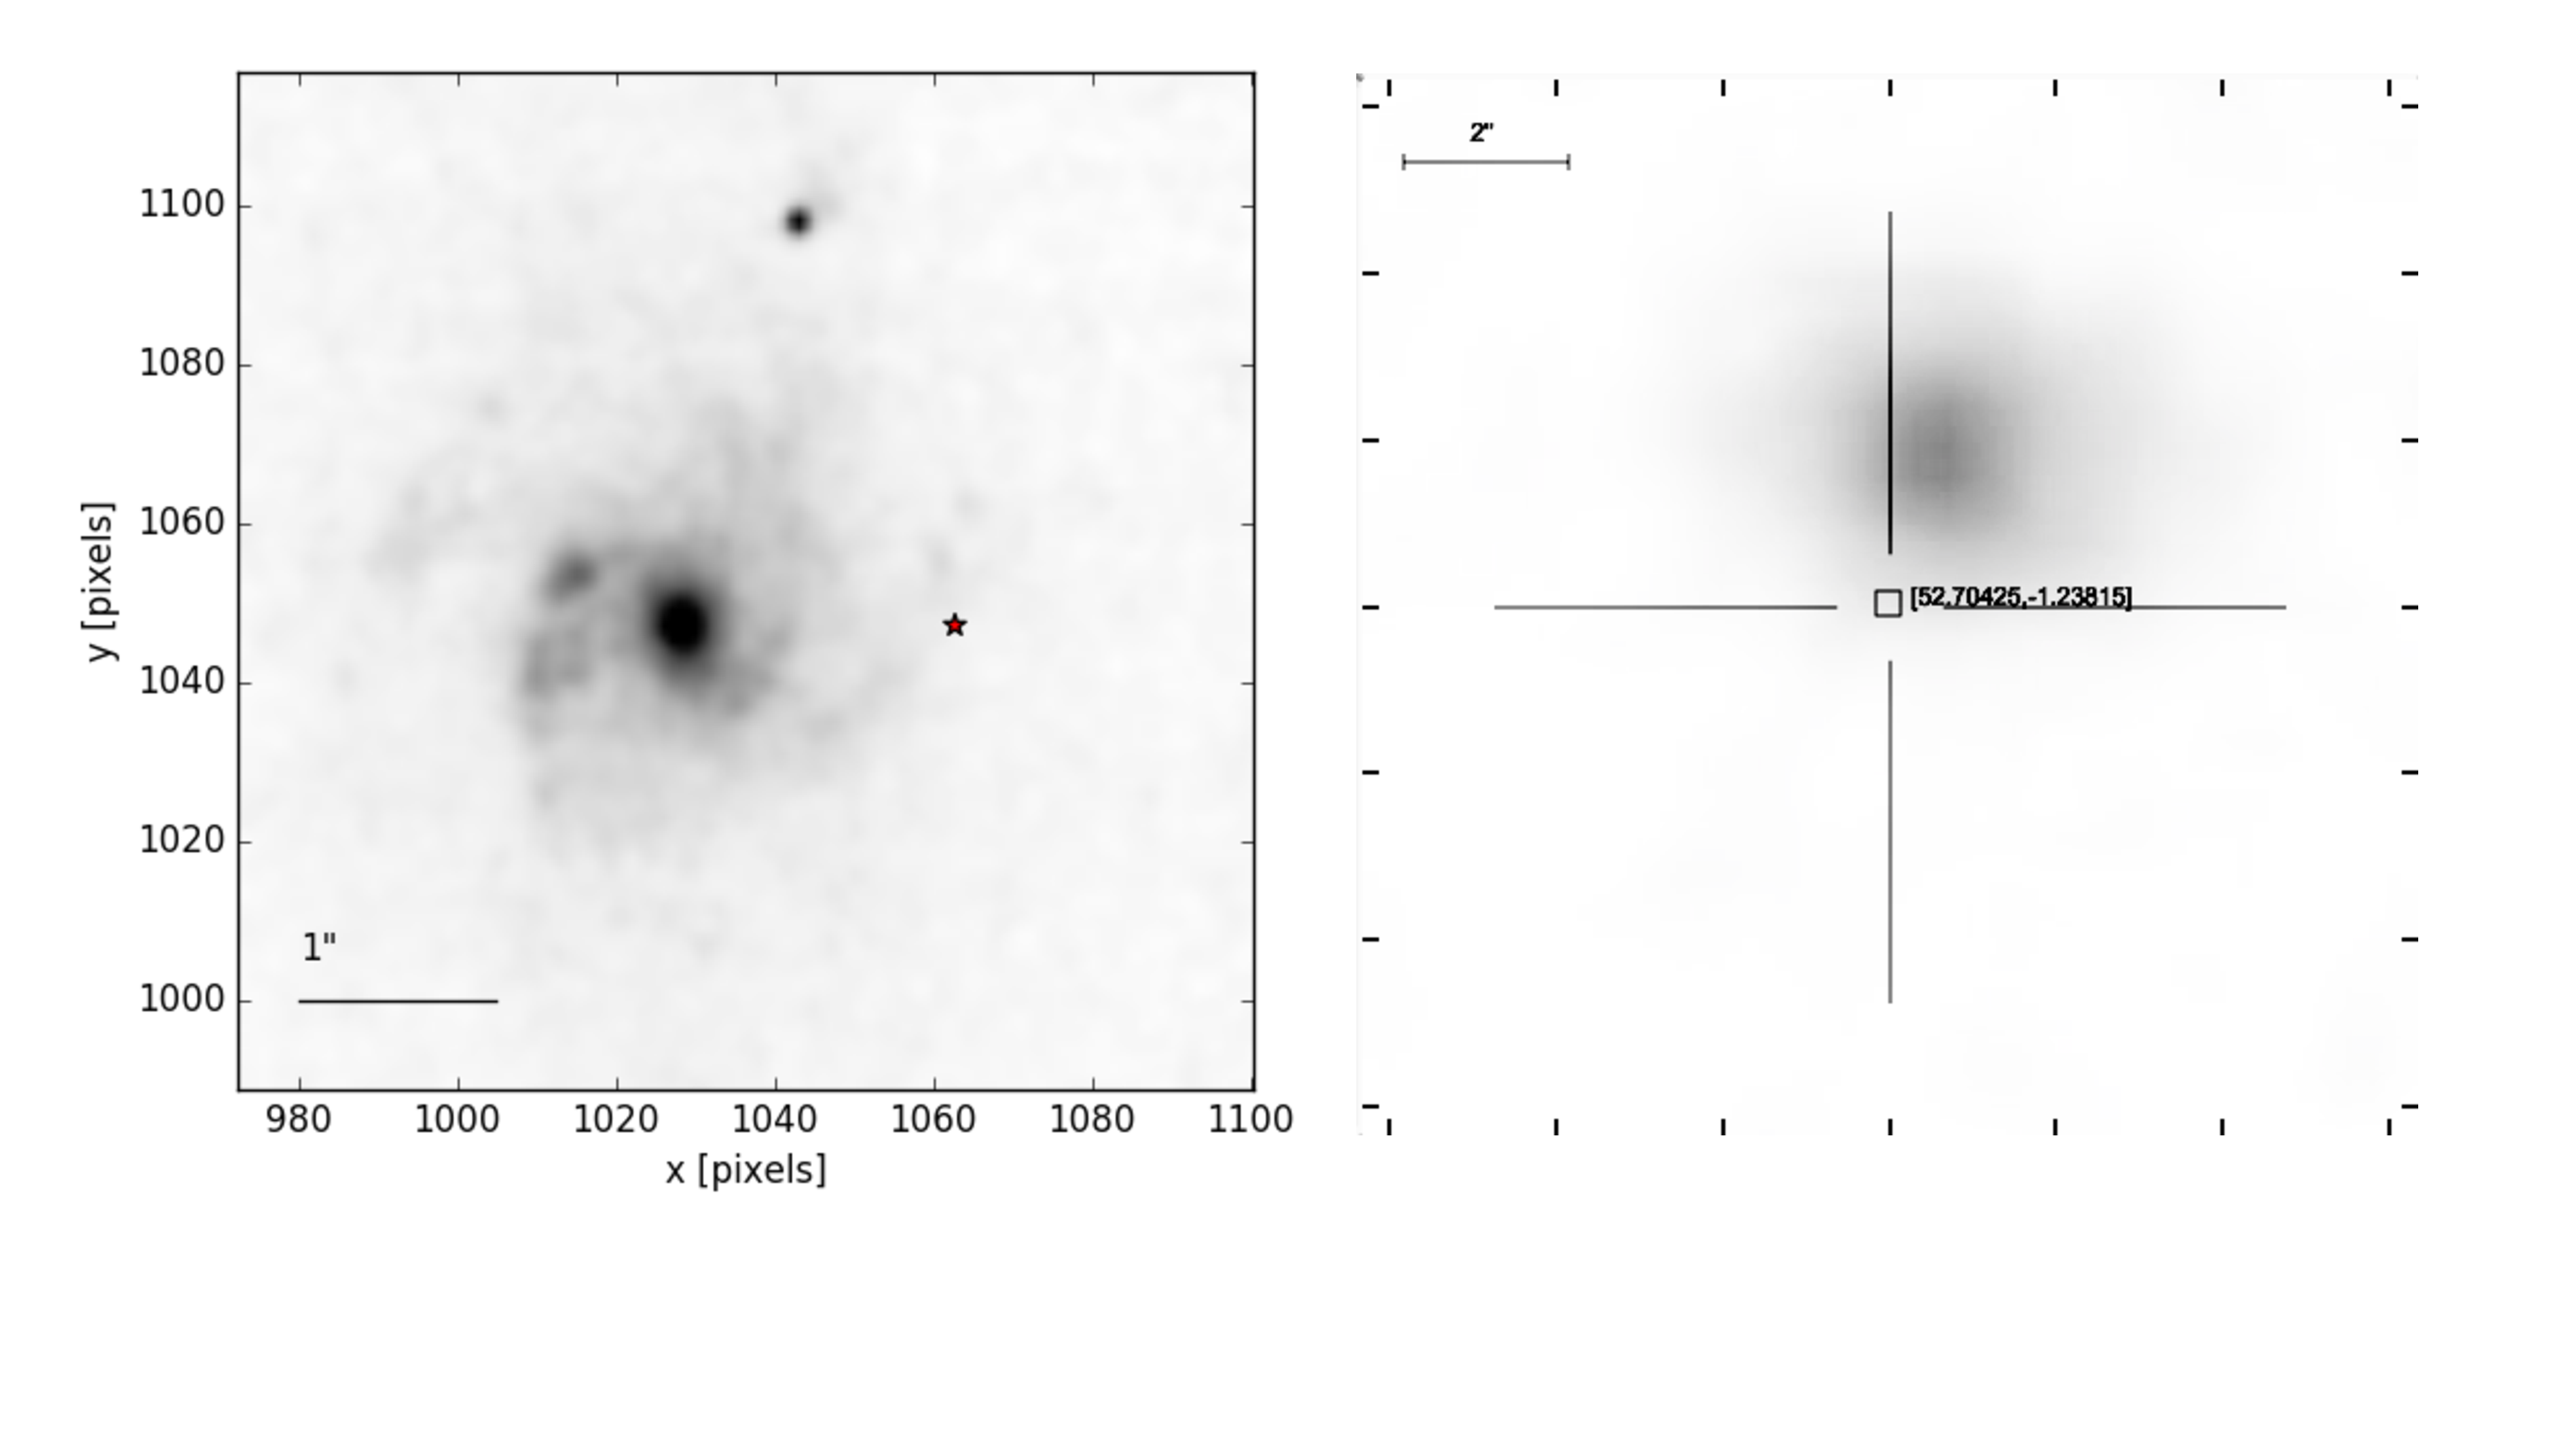
\includegraphics[width=3.5in]{SN2635-combined-inverted.pdf}
	\caption{Host galaxy of SDSS SN2635 (SN 2005fw), at a redshift of $z=0.143$. HST 
	(left) one pixel is $114~\text{pc}$, and SDSS (right) one pixel is $1,140~\text{pc}$.}
	\label{f:galaxy-compare}
\end{figure}

This process is not new, but HST's resolution allows us to probe hosts at a
higher redshift. These redshifts are needed because the residuals on the Hubble
diagram will allow for analysis of systematics and not be dominated by bulk
motion. The redshift range of SDSS-II Supernovae Survey is $z=0.05-0.4$. The HST
observations were taken in two filters, with $360~\text{second}$ exposures each.

After processing and analysis, the HST images will produce several variables
describing the local environments of the \sn{}. These variables will be compared
to the \sn{}'s absolute brightness and residual on the Hubble diagram for
correlations. The first of these variables being the \sn{}'s fractional pixel
rank (FPR). The FPR is the ranked fraction, by brightness, of the pixel at the
\sn{}'s position relative to the rest of the galaxy. This gives us a proxy for
star formation. Another variable would be the color of the \sn{}'s pixel. Color
can give a idea of the age of stars in that region. Further analysis of subsets
can also be done and questions like whether there is a bias for \sn{} in clumpy
regions of elliptical galaxies can be answered.

% F derivative R - (second derivative) - finds things that do not match 
% its neighbors (nor follows a nice smooth slope like ellipticals)
% a color - Yea color-mag diagram \& ``type/max age'' of stellar region

\subsection{Beyond HST}\label{beyond-hst}

Difficulties in this analysis will all come from the data itself. The most
obvious issue is that there are only 61 host galaxies, compared to around 1000
\sn{} seen with SDSS \citep{Campbell13}. There is a large number of targets
that still could be observed to increase the data set and improve our
statistical uncertainties. More HST observations would be optimal, because of
its high angular resolution in the visible. Ground based infrared photometry
with adoptive optics would produce a meaningful data set, but it would be
difficult to add it to our current optical data.

I can get more data in several other ways. SDSS-IV's MaNGA is using integrated
field units (IFUs) to get spectra at spacial scales of $\sim 2 ~\text{kpc}$ and
they have a call for ancillary proposals coming out this fall. Even though MaNGA
has large angular resolution, IFU's are a common technique and their resolution
will only get smaller with time. Alternative IFU's can be used, including Keck
OSIRIS which observes in the infrared with a spacial element similar to HST
($0.020'' - 0.100''$) \citep{OSIRIS},
% \url{http://ifs.wikidot.com/instruments#toc12})  
or Gemini GMOS which observes in the optical but has a much larger resolution
$0.2''$ \citep{Gemini}.
% \url{http://ifs.wikidot.com/instruments#toc7}) 

The angular resolution of HST would not be as necessary if we observed host
galaxies of local \sn{}, but these observations also have issues. First, the
number of \sn{} is proportional to the volume for which you are looking, and
there is more volume at higher redshift. Secondly,
% there are questions about whether \sn{} are the same across cosmic time, so 
with a concern for a bias in \Hubble{} due to anchoring only a subtype of \sn{} 
these local environment tests should be done for
as wide a range of redshifts as possible. For these reasons, SDSS's $z \sim 0.1$
is a good redshift to perform these tests. At this redshift, HST's high angular
resolution is the best for observing a true local environment.

\section{Conclusion}

\sn{} have been a standard cosmological tool for decades. In this time their
absolute magnitude has been continually refined to be more precise and
standardized. Now \sn{} detections are numerous enough and their distances are
accurate enough to start testing the Cosmological Principle and looking for a
bias in the Hubble constant. These two tests are complementary.  The next
step in searching for a cosmic-scale bulk flow is to lower the statistical
uncertainties of \sn{}. This will be done by future large scale surveys but
their impact needs to be understood through simulations or their usefulness will
be limited.  The next step for testing for a bias in \Hubble{} is to lower \sn{}
systematic uncertainties. These uncertainties appear to be correlated with local
environments, but the exact variable is still unknown. More high resolution
observations need to be done allowing for a thorough analysis of the local
environment's effects on \sn{}.

%  The objectives of this research
% are to continue the analysis of \sn{} calibration and the search of a cosmic-
% scale bulk flow. 
% The next step in searching for a cosmic-scale bulk flow is to
% simulate and fully understand what is knowable from future surveys like LSST.
% The next step for \sn{} calibration is to more fully understand the local
% environment.

\bibliographystyle{apj}
\bibliography{2016-02-07-w-ResearchProposal}

\end{document}